% ***************************************************************************************
% ************************************* CAPÍTULO I **************************************
% ***************************************************************************************
\chapter{** TITULO DEL CAPÍTULO 1 **}
\thispagestyle{empty}

\abovedisplayskip=0pt
\belowdisplayskip=10pt
\abovedisplayshortskip=0pt
\belowdisplayshortskip=10pt

** COLOQUE AQUÍ CONTENIDO RESPECTIVO **

** A CONTINUACIÓN SE HACE UN RESUMEN DE LAS PRINCIPALES HERRAMIENTAS NECESARIAS PARA ESCRIBIR SU LIBRO DE PROYECTO DE GRADO. EL OBJETIVO DE ESTO ES AHORRAR LA MAYOR CANTIDAD DE TIEMPO EN EL \textit{LAYOUT}, ENFOCANDO LOS ESFUERZOS EN EL CONTENIDO DEL PROYECTO **

\section{Figures}

\subsection{Referenciado y posicionamiento de imagenes}

En la figura \ref{fig:cromovegetal} se observa el jardín cromovegetal, concebido por Carlos Cruz-Diez en 1991 en su visita a la Universidad Simón Bolívar.

% for a correct image positioning is important to use the parameters [H], [h] and [p] in a right way.
% The first one place the image in the exact position that is in the LaTeX code
% The second one place the image where the compiler configurate as "best position"
% The last one utilize an entire page for figure positioning

\begin{figure}[H]
\centering
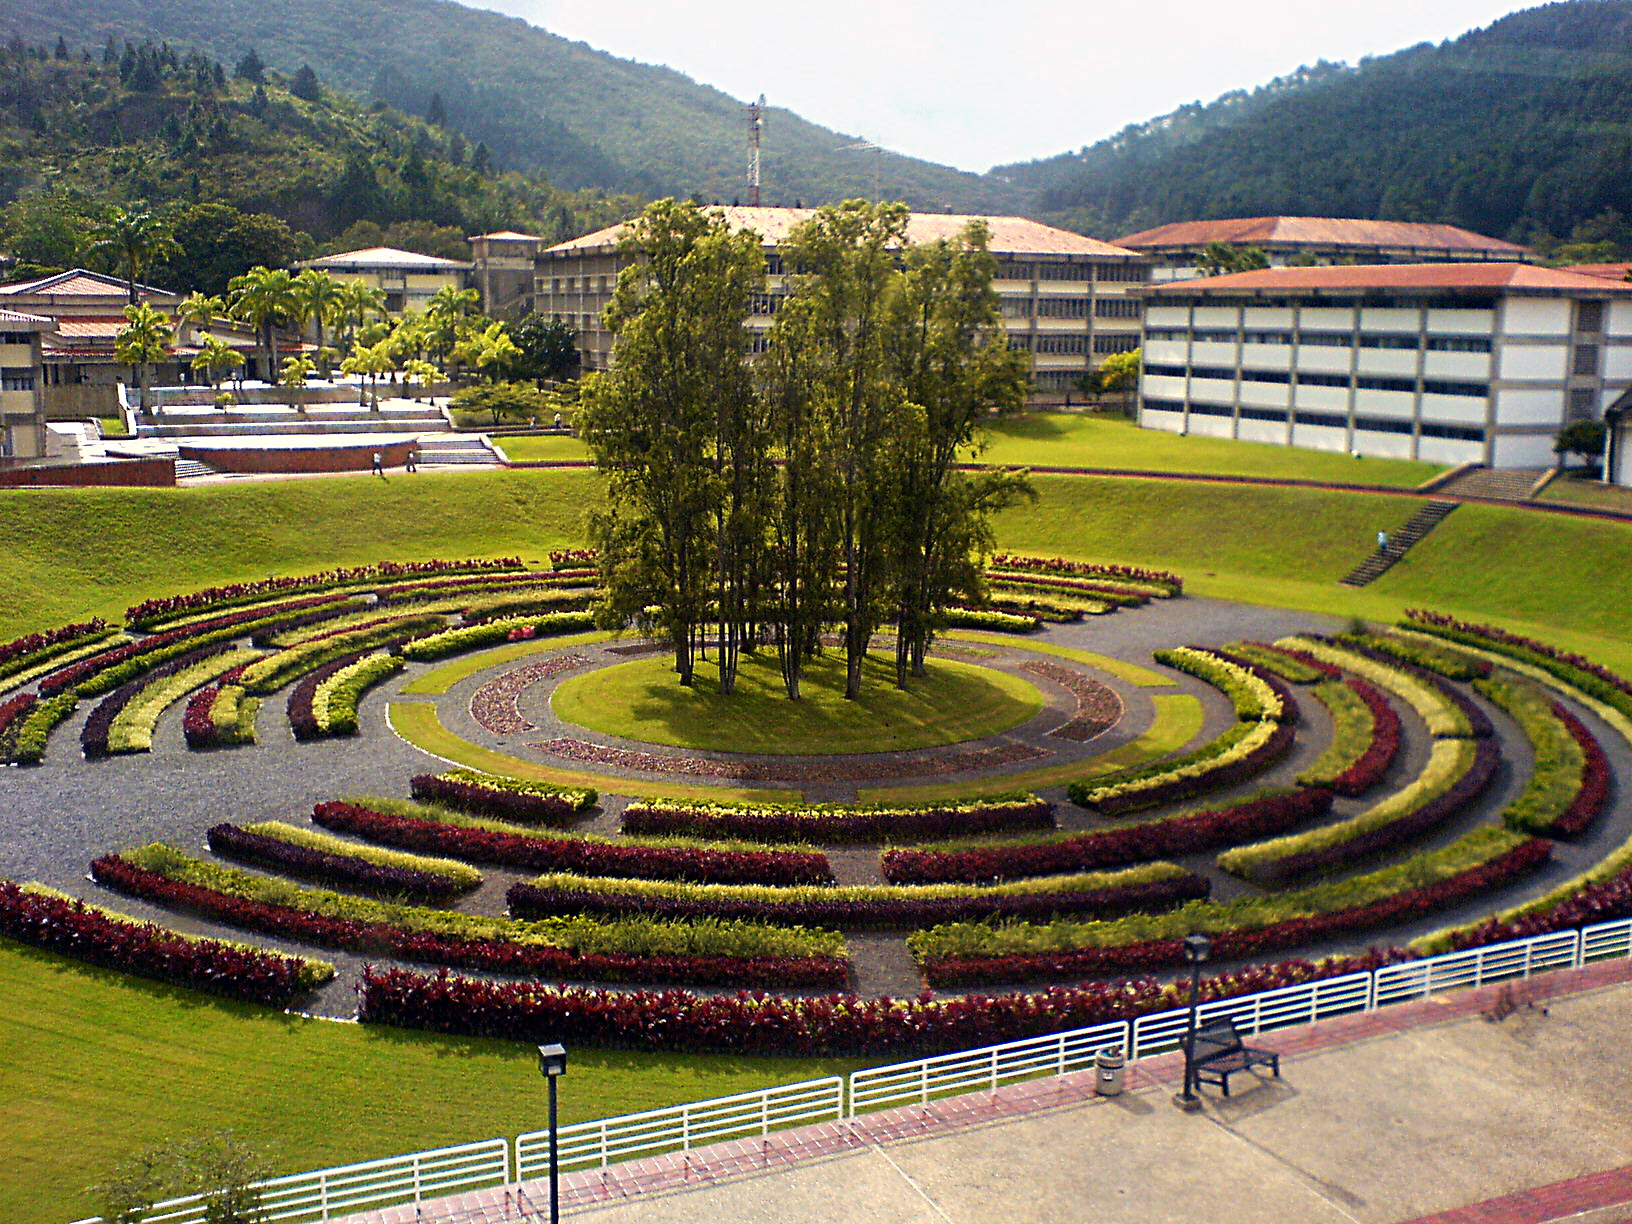
\includegraphics[width=0.50\textwidth]{2_MainMatter/Capitulo1/Imagenes/cromovegetal.jpg}
\caption{Jardín cromovegetal de la Universidad Simón Bolívar}
\label{fig:cromovegetal}
\end{figure}

\subsection{Ejemplo de posicionamiento en hoja completa}

La figura \ref{fig:rectorado} muestra el rectorado de la Universidad Simón Bolívar, sede de los principales entes administrativos de la institución.

\begin{figure}[p]
\centering
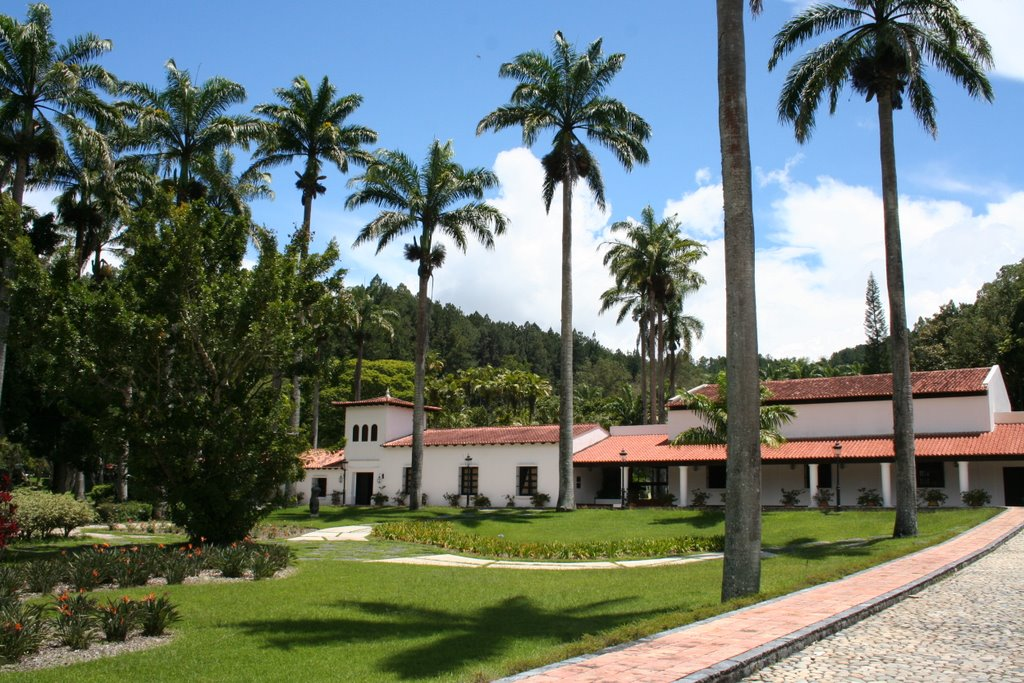
\includegraphics[width=1.0\textwidth]{2_MainMatter/Capitulo1/Imagenes/rectorado.jpg}
\caption{Rectorado de la Universidad Simón Bolívar}
\label{fig:rectorado}
\end{figure}

\subsection{Ángulo de giro en imágenes con orientación horizontal}

La figura \ref{fig:biblioteca} muestra la biblioteca de la USB, lugar de estudio e investigación de un gran número de miembros de la comunidad universitaria.

\begin{figure}[p]
\centering
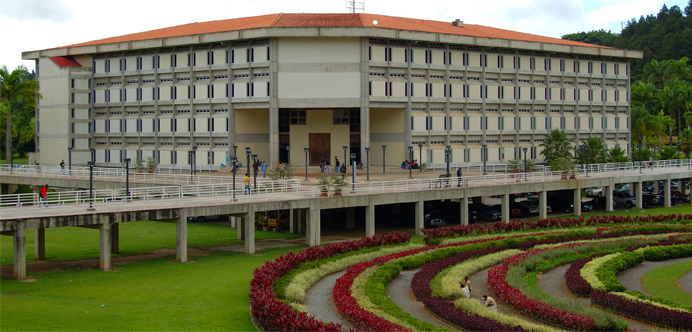
\includegraphics[width=1.3\textwidth, angle=90]{2_MainMatter/Capitulo1/Imagenes/biblioteca.jpg}
\caption{Biblioteca de la Universidad Simón Bolívar}
\label{fig:biblioteca}
\end{figure}

\section{listas}

A continuación se enumeran las partes que debe tener el libro de proyecto de grado:

\begin{enumerate}
    \item Carátula.
    \item Página de título.
    \item Acta final de evaluación.
    \item Resumen.
    \item Página de dedicatoria (opcional).
    \item Agradecimientos (opcional).
    \item Índice general.
    \item Índice de tablas (si las hay).
    \item Índice de figuras (si las hay).
    \item Índice de símbolos (si los hay).
    \item Índice de abreviaturas (si los hay).
    \item Introducción.
    \item Cuerpo del trabajo:
    \begin{itemize}
        \item Capítulo 1.
        \item Capítulo 2.
        \item ...
        \item Capítulo N.
    \end{itemize}
    \item Conclusiones y recomendaciones.
    \item Referencias.
    \item Apéndices.
\end{enumerate}

\section{Quotes}

Existen dos tipos de citas textuales, cada una con su forma para representarlas en el libro.

\subsection{Menores a 3 líneas}

La Universidad Simón Bolívar es reconocida internacionalmente \textquote{como un centro de excelencia por su capacidad de formar líderes con un alto compromiso social, por su capacidad de generar aportes creativos y pertinentes de naturaleza tecnológica, científica y humana}.

\subsection{Mayores a 3 líneas}

La misión de la Universidad Simón Bolívar, detallada en \url{http://www.usb.ve/home/node/33}, queda estipulada como:

\begin{displayquote}
La Universidad Simón Bolívar es una comunidad académica, innovadora, participativa, productiva y plural, en permanente aprendizaje y desarrollo, y comprometida con la excelencia, cuya misión fundamental es contribuir significativamente con: la formación sustentada en valores éticos de ciudadanos libres, líderes emprendedores, de alta calidad profesional y humana, orientados hacia la creatividad, la innovación, la producción, la sensibilidad y la solidaridad social; la búsqueda y transmisión universal del saber, la generación, difusión y aplicación del conocimiento; dentro de un foro libre, abierto y crítico; la transferencia directa de su labor investigativa, académica, creativa y productiva, a manera de soluciones y respuestas a las necesidades y demandas de la sociedad, a cuyo servicio se encuentra, en pos de un mundo mejor.
\end{displayquote}

\section{Tables}

Para generar tablas de forma rápida me gusta utilizar un entorno gráfico como \url{http://www.tablesgenerator.com/}. En la tabla \ref{table:power_values} se presenta una estructura de ejemplo a partir de la cual se puede tener una primera aproximación. \textit{adjustbox} ajusta el tamaño de la tabla al formato de página utilizado.

\begin{table}[h]
\centering
\caption{Valores de potencia recibida en escenario con línea de vista}
\label{table:power_values}
\begin{adjustbox}{width=1\textwidth}
\small
\begin{tabular}{|c|c|c|c|c|c|c|c|c|}
\hline
\rowcolor[HTML]{C0C0C0} 
{\color[HTML]{000000} \textbf{\begin{tabular}[c]{@{}c@{}}Número de\\ medición\end{tabular}}}             & {\color[HTML]{000000} \textbf{\begin{tabular}[c]{@{}c@{}}1 m\\ {[}dBm{]}\end{tabular}}} & {\color[HTML]{000000} \textbf{\begin{tabular}[c]{@{}c@{}}10 m\\ {[}dBm{]}\end{tabular}}} & {\color[HTML]{000000} \textbf{\begin{tabular}[c]{@{}c@{}}30 m\\ {[}dBm{]}\end{tabular}}} & {\color[HTML]{000000} \textbf{\begin{tabular}[c]{@{}c@{}}50 m\\ {[}dBm{]}\end{tabular}}} & \textbf{\begin{tabular}[c]{@{}c@{}}70 m\\ {[}dBm{]}\end{tabular}} & \textbf{\begin{tabular}[c]{@{}c@{}}90 m\\ {[}dBm{]}\end{tabular}} & \textbf{\begin{tabular}[c]{@{}c@{}}110 m\\ {[}dBm{]}\end{tabular}} & \textbf{\begin{tabular}[c]{@{}c@{}}130 m\\ {[}dBm{]}\end{tabular}}
\\ \hline
\rowcolor[HTML]{EFEFEF} 
\cellcolor[HTML]{C0C0C0}{\color[HTML]{000000} \textbf{1}}      & -52                                                                                     & -68                                                                                      & -81                                                                                      & -78                                                                                      & -86                                                               & -87                                                               & -90                                                               & -93
\\ \hline
\cellcolor[HTML]{C0C0C0}{\color[HTML]{000000} \textbf{2}}      & -52                                                                                     & -68                                                                                      & -75                                                                                      & -78                                                                                      & -87                                                               & -87                                                               & -93                                                               & -93
\\ \hline
\rowcolor[HTML]{EFEFEF} 
\cellcolor[HTML]{C0C0C0}{\color[HTML]{000000} \textbf{3}}      & -52                                                                                     & -67                                                                                      & -73                                                                                      & -81                                                                                      & -81                                                               & -88                                                               & -89                                                              & -92
\\ \hline
\cellcolor[HTML]{C0C0C0}{\color[HTML]{000000} \textbf{4}}      & -48                                                                                     & -67                                                                                      & -73                                                                                      & -81                                                                                      & -81                                                               & -87                                                               & -91                                                               & -93 
\\ \hline
\rowcolor[HTML]{EFEFEF} 
\cellcolor[HTML]{C0C0C0}{\color[HTML]{000000} \textbf{5}}      & -59                                                                                     & -67                                                                                      & -73                                                                                      & -86                                                                                      & -82                                                               & -87                                                               & -91                                                               & -92
\\ \hline
\cellcolor[HTML]{C0C0C0}{\color[HTML]{000000} \textbf{6}}      & -60                                                                                     & -67                                                                                      & -73                                                                                      & -81                                                                                      & -83                                                               & -88                                                               & -91                                                               & -92
\\ \hline
\rowcolor[HTML]{EFEFEF} 
\cellcolor[HTML]{C0C0C0}\textbf{7}                             & -61                                                                                     & -67                                                                                      & -73                                                                                      & -81                                                                                      & -85                                                               & -90                                                               & -91                                                               & -93
\\ \hline
\cellcolor[HTML]{C0C0C0}\textbf{8}                             & -61                                                                                     & -65                                                                                     & -74                                                                                      & -79                                                                                      & -85                                                               & -90                                                               & -92                                                               & -93
\\ \hline
\rowcolor[HTML]{EFEFEF} 
\cellcolor[HTML]{C0C0C0}\textbf{9}                             & -61                                                                                     & -67                                                                                      & -75                                                                                      & -79                                                                                      & -84                                                               & -89                                                               & -92                                                               & -92
\\ \hline
\cellcolor[HTML]{C0C0C0}\textbf{10}                            & -63                                                                                     & -68                                                                                      & -76                                                                                      & -78                                                                                      & -87                                                               & -90                                                               & -92                                                               & -93
\\ \hline
\rowcolor[HTML]{C0C0C0} 
{\color[HTML]{000000} \textbf{Media $(\mu)$}}                  & {\color[HTML]{000000} \textbf{-56,90}}                                                     & {\color[HTML]{000000} \textbf{-67,10}}                                                      & {\color[HTML]{000000} \textbf{-74,60}}                                                      & {\color[HTML]{000000} \textbf{-80,20}}                                                      & \textbf{-84,10}                                                      & \textbf{-88,30}                                                      & \textbf{-91,20}                                                      & \textbf{-92,60}
\\ \hline
\rowcolor[HTML]{C0C0C0} 
{\color[HTML]{000000} \textbf{\begin{tabular}[c]{@{}c@{}}Desviación\\ Estándar $(\sigma)$\end{tabular}}} & {\color[HTML]{000000} \textbf{-5,30}}                                                     & {\color[HTML]{000000} \textbf{-0,88}}                                                      & {\color[HTML]{000000} \textbf{-2,50}}                                                      & {\color[HTML]{000000} \textbf{-2,44}}                                                      & \textbf{-2,28}                                                      & \textbf{-1,34}                                                      & \textbf{-1,14}                                                      & \textbf{-0,52}
\\ \hline
\end{tabular}
\end{adjustbox}
\end{table}https://www.overleaf.com/project/5ee251987e42b100016458e6

\section{Equations}

La ecuación \ref{eq:newton_second_law} establece la segunda ley de newton:

\begin{equation}
    F_{net} = M \times a
\label{eq:newton_second_law}
\end{equation}

\section{Programming Code}

Aunque no es común agregar códigos de programación en los capítulos del trabajo de grado (si es necesario se deben colocar como apéndices del mismo), a continuación una primera aproximación mediante un simple programa \textit{Hola Mundo}. La asignación de colores para cada tipo de instrucción es configurable en el archivo de preámbulo.

\begin{lstlisting}[language=C]
// just a "Hello World" program
#include <stdio.h>

void main(){
    printf("Hello World");
}
\end{lstlisting}

\section{Referencias}

Para más información, \textit{Hints and Tips on (Science and Engineering) Bachelor’s and Master’s Thesis Writing} \cite{Thesis_LaTeX_2} y \textit{Writing a thesis with LaTeX} \cite{Thesis_LaTeX} tienen consejos y recomendaciones relevantes.
